\documentclass[journal]{IEEEtran}
\usepackage{cite}
\usepackage{amsmath,amssymb,amsfonts}
\usepackage{algorithmic}
\usepackage{graphicx}
\usepackage{textcomp}
\usepackage{xcolor}
\usepackage{url}
\usepackage{hyperref}
\usepackage{tikz}
\usetikzlibrary{shapes.geometric, arrows.meta, positioning, fit, backgrounds, calc}

\begin{document}

\title{Identity-Centric Zero Trust Architecture: A Comprehensive Framework for Modern Enterprise Security Governance}

\author{Ezekiel Ologunde%
\thanks{E. Ologunde is an independent researcher and Doctoral Student in Cybersecurity Analytics at the School of Engineering and Applied Science, The George Washington University, Washington, DC 20052}}

\markboth{ }{Ologunde: Identity-Centric Zero Trust Architecture}

\maketitle

\begin{abstract}
The traditional perimeter-based security paradigm, predicated on implicit trust within
organizational networks, has proven inadequate in the face of sophisticated supply chain
attacks and insider threats, as evidenced by recent breaches including SolarWinds and
Colonial Pipeline. This paper presents a comprehensive framework for implementing
Identity, Credential, and Access Management (ICAM)-enabled Zero Trust Architecture (ZTA)
that fundamentally shifts the security paradigm from network-centric to identity-centric
protection. We examine the critical architectural scope considerations for Zero Trust
implementation, emphasizing risk-based prioritization of high-value assets and the
governance role of modern ICAM solutions. Through analysis of centralized versus
federated identity structures, we demonstrate how architectural decisions impact security
posture, operational flexibility, and regulatory compliance across diverse organizational
contexts. Our framework integrates three core ICAM capabilities---strong authentication
and federation, governance and lifecycle management, and continuous monitoring
analytics---as foundational elements enabling the ``never trust, always verify''
principle. We address the unique challenges facing small and medium enterprises (SMEs)
in adopting Zero Trust, proposing graduated implementation strategies aligned with
business objectives and resource constraints. The research synthesizes contemporary
cybersecurity frameworks including NIST Special Publication 800-207, empirical studies
on risk management maturity, and real-world implementation experiences from government
and commercial sectors.
\end{abstract}

\begin{IEEEkeywords}
Zero Trust Architecture, Identity and Access Management, ICAM, cybersecurity governance,
federated identity, centralized identity, risk-based security, continuous verification,
least privilege access
\end{IEEEkeywords}

\section{Introduction}
\IEEEPARstart{F}{or} decades, enterprise cybersecurity architectures operated under a
fundamental assumption that proved increasingly untenable: threats originate primarily
from outside the organizational network perimeter, and entities within that perimeter
merit implicit trust. This ``castle-and-moat'' paradigm dominated security thinking
throughout the early internet era, with organizations investing heavily in firewalls,
intrusion detection systems, and virtual private networks designed to establish clear
boundaries between trusted internal networks and untrusted external
environments~\cite{rose2020zero}.

However, high-profile incidents including the 2020 SolarWinds supply chain compromise
and the 2021 Colonial Pipeline ransomware attack demonstrate that threats increasingly
originate from within nominally trusted environments~\cite{nist800207}. Simultaneously,
cloud adoption, remote workforce proliferation, and IoT deployments have eroded the
viability of perimeter-based models such that the concept of a defined network perimeter
becomes increasingly meaningless~\cite{pingidentity2024}.

Zero Trust Architecture (ZTA) emerged as a response, inverting the security paradigm
from ``trust but verify'' to ``never trust, always verify.'' As Rose et al.\ articulate
in NIST SP 800-207, Zero Trust ``assumes that a breach is inevitable or has likely
already occurred,'' requiring continuous verification and least-privilege access
enforcement~\cite{rose2020zero}. Central to Zero Trust's effectiveness is ICAM---the
suite of capabilities enabling organizations to verify identities, manage access rights,
and continuously monitor for anomalous behavior. In a Zero Trust architecture, identity
becomes the new perimeter~\cite{pingidentity2024}.

\subsection{Research Contributions}

This paper provides: (1)~a risk-based methodology for defining Zero Trust architectural
scope; (2)~analysis of how ICAM capabilities enable Zero Trust governance; (3)~comparative
evaluation of centralized versus federated identity structures with decision criteria;
(4)~practical SME adoption guidance; and (5)~integration of empirical risk management
research with Zero Trust principles.

\section{Background and Related Work}

\subsection{Evolution of Zero Trust Concepts}

The term ``Zero Trust'' was coined by Forrester Research analyst John Kindervag in
2010~\cite{kindervag2010}. NIST formalized Zero Trust principles in SP~800-207,
identifying seven core tenets including: all communication is secured regardless of
network location; access is granted per-session based on dynamic policy; all
authentication and authorization are dynamic and strictly enforced; and the enterprise
collects continuous intelligence to improve security posture~\cite{rose2020zero}.

\subsection{Identity, Credential, and Access Management}

The Federal CIO Council defines ICAM as ``the set of tools, policies, and systems that
allow an organization to manage, monitor, and secure access to protected
resources''~\cite{ficam2021}. Core ICAM functions include identity management,
credential management, access management, and governance. Federation enables users from
one organization to access resources in another using their home credentials via trust
frameworks (SAML, OAuth~2.0, OIDC, FIDO)~\cite{pingidentity2024}.

\subsection{Risk-Based Security Architectures}

Shimizu and Hashimoto~\cite{shimizu2025vulnerability} developed vulnerability management
frameworks using exploit prediction data, demonstrating that prioritizing based on
real-world exploitation probability significantly reduces mean time to remediation. The
FAIR Institute's 2025 report provides empirical evidence that organizations employing
quantitative risk assessment achieve 37\% more effective cybersecurity budget
allocation~\cite{fairinstitute2025}. Chang et al.~\cite{chang2025mind} identify
leadership awareness as a critical barrier in SMEs, finding 67\% of decision-makers
significantly underestimate cyber risk. Campos et al.~\cite{campos2025safeguarding}
found that gradual implementation tied to specific business objectives yields superior
outcomes compared to disruptive comprehensive deployments.

\begin{figure}[!t]
\centering
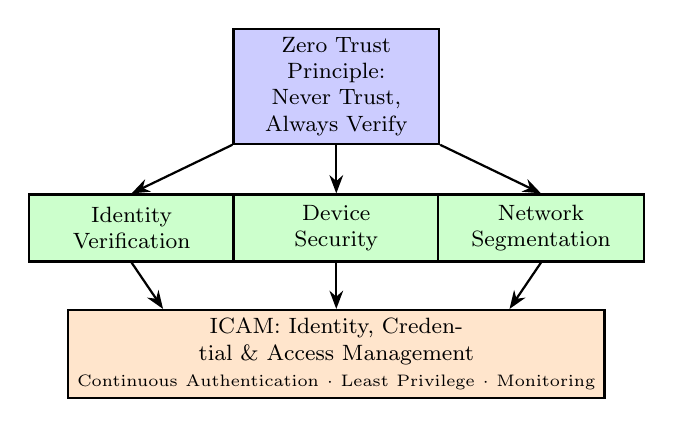
\begin{tikzpicture}[
  font=\footnotesize,
  >=Stealth,
  box/.style={rectangle, draw, thick, minimum width=2.6cm, minimum height=0.85cm,
              align=center, text width=2.4cm, inner sep=3pt},
  arr/.style={-{Stealth}, thick}
]
  %% Core principle at top
  \node[box, fill=blue!20] (principle) at (0,0)
    {Zero Trust Principle:\\Never Trust,\\Always Verify};

  %% Three pillars below, explicit coordinates
  \node[box, fill=green!20] (identity) at (-2.6,-1.8) {Identity\\Verification};
  \node[box, fill=green!20] (device)   at (  0.0,-1.8) {Device\\Security};
  \node[box, fill=green!20] (network)  at ( 2.6,-1.8) {Network\\Segmentation};

  %% ICAM bar at bottom — fixed width 6.8cm centred at x=0
  \node[box, fill=orange!20, minimum width=6.8cm, minimum height=0.85cm,
        text width=6.6cm] (icam) at (0,-3.4)
    {ICAM: Identity, Credential \& Access Management\\
     \fontsize{6.5pt}{8pt}\selectfont
     Continuous Authentication $\cdot$ Least Privilege $\cdot$ Monitoring};

  %% Arrows from principle to pillars
  \draw[arr] (principle.south west) -- (identity.north);
  \draw[arr] (principle.south)      -- (device.north);
  \draw[arr] (principle.south east) -- (network.north);

  %% Arrows from pillars to ICAM
  \draw[arr] (identity.south) -- ([xshift=-2.2cm]icam.north);
  \draw[arr] (device.south)   -- (icam.north);
  \draw[arr] (network.south)  -- ([xshift= 2.2cm]icam.north);
\end{tikzpicture}
\caption{Zero Trust Architecture pillars supported by ICAM. The ``never trust, always
  verify'' principle manifests through identity verification, device security posture
  assessment, and network micro-segmentation, all governed by ICAM capabilities.}
\label{fig:zt_pillars}
\end{figure}

\section{Defining Zero Trust Architectural Scope: A Risk-Based Framework}

Attempting to implement Zero Trust across all enterprise systems simultaneously overwhelms
resources and delays benefits. We propose a four-phase risk-based framework.

\subsection{Phase 1: Identify and Prioritize Crown Jewels}

Organizations begin by identifying systems, data, and capabilities whose compromise would
cause maximum organizational damage: intellectual property, financial systems, customer
data, operational control systems, and administrative access. Crown jewels are prioritized
by exposure, attractiveness to adversaries, current protection adequacy, and impact
severity from compromise.

\subsection{Phase 2: Define Protection Boundaries}

For prioritized assets, organizations define: the subject population requiring access
(employees, contractors, automated systems); the resource inventory to protect; and
legitimate access patterns forming behavioral baselines enabling anomaly detection.

\subsection{Phase 3: Implement Zero Trust Controls}

Controls include: multi-factor authentication (FIDO2/PKI for highest-risk scenarios);
least-privilege access with just-in-time privilege escalation; micro-segmentation
preventing lateral movement; and continuous monitoring integrated with SIEM/UEBA.

\subsection{Phase 4: Expand Scope Incrementally}

As initial implementations mature, organizations expand to next-most-critical assets,
following risk-based prioritization. This aligns with Shimizu and
Hashimoto~\cite{shimizu2025vulnerability}, who demonstrate focused prioritization yields
superior outcomes compared to attempting comprehensive coverage immediately.

\begin{figure*}[!t]
\centering
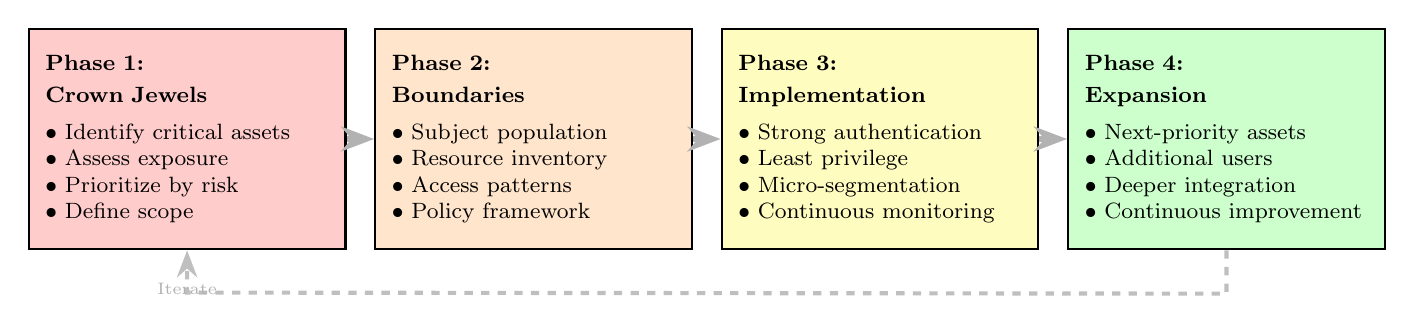
\begin{tikzpicture}[
  font=\footnotesize,
  >=Stealth,
  sbox/.style={
    rectangle, draw, thick,
    minimum width=3.8cm, minimum height=2.8cm,
    align=left, text width=3.6cm, inner sep=6pt
  },
  arr/.style={-{Stealth}, line width=2pt}
]
  %% Four stages at explicit x-positions; gap = 0.6cm; box width 3.8cm
  %% Centres: 0, 4.4, 8.8, 13.2 → right edge = 13.2+1.9 = 15.1cm ✓
  \node[sbox, fill=red!20]    (p1) at (0,0) {
    \textbf{Phase 1:}\\[2pt]\textbf{Crown Jewels}\\[4pt]
    $\bullet$ Identify critical assets\\
    $\bullet$ Assess exposure\\
    $\bullet$ Prioritize by risk\\
    $\bullet$ Define scope
  };
  \node[sbox, fill=orange!20] (p2) at (4.4,0) {
    \textbf{Phase 2:}\\[2pt]\textbf{Boundaries}\\[4pt]
    $\bullet$ Subject population\\
    $\bullet$ Resource inventory\\
    $\bullet$ Access patterns\\
    $\bullet$ Policy framework
  };
  \node[sbox, fill=yellow!25] (p3) at (8.8,0) {
    \textbf{Phase 3:}\\[2pt]\textbf{Implementation}\\[4pt]
    $\bullet$ Strong authentication\\
    $\bullet$ Least privilege\\
    $\bullet$ Micro-segmentation\\
    $\bullet$ Continuous monitoring
  };
  \node[sbox, fill=green!20]  (p4) at (13.2,0) {
    \textbf{Phase 4:}\\[2pt]\textbf{Expansion}\\[4pt]
    $\bullet$ Next-priority assets\\
    $\bullet$ Additional users\\
    $\bullet$ Deeper integration\\
    $\bullet$ Continuous improvement
  };

  %% Forward arrows
  \draw[arr, gray!60] (p1.east)--(p2.west);
  \draw[arr, gray!60] (p2.east)--(p3.west);
  \draw[arr, gray!60] (p3.east)--(p4.west);

  %% Feedback arc below all boxes
  \draw[-{Stealth}, line width=1.5pt, dashed, gray!50]
    (p4.south) -- ++(0,-0.55)
    -- (0, -1.95)
    -- (p1.south)
    node[midway, below, font=\fontsize{6.5pt}{8pt}\selectfont, text=gray!60]
    {Iterate};
\end{tikzpicture}
\caption{Four-phase risk-based framework for Zero Trust scope definition. Organizations
  begin with crown jewel identification, define protection boundaries, implement controls,
  and incrementally expand scope following risk-based prioritization.}
\label{fig:zt_phases}
\end{figure*}

\section{ICAM as Zero Trust Governance Foundation}

ICAM provides the governance foundation through three core capability areas.

\subsection{Strong Authentication and Federation}

Modern Zero Trust requires phishing-resistant MFA such as FIDO2 security keys or PKI
certificates that cryptographically bind authentication to specific
devices~\cite{cisa2024mfa}. Risk-adaptive authentication dynamically adjusts requirements
based on device posture, network location, behavioral patterns, and resource sensitivity.
Federation enables Zero Trust across organizational boundaries---as exemplified by NASA's
implementation spanning centers, contractors, and international partners while maintaining
consistent policy enforcement~\cite{pingidentity2024}.

\subsection{Governance and Lifecycle Management}

ICAM governs identity throughout its lifecycle: automated provisioning ensures consistency
during onboarding; periodic access reviews verify least privilege; and timely
deprovisioning prevents orphaned accounts. Centralized policy (RBAC, ABAC, least
privilege, separation of duties, time-based access) ensures consistency across diverse
resources. Privileged Access Management capabilities---just-in-time elevation, session
recording, credential vaulting, and break-glass procedures---address the highest-value
attacker targets.

\subsection{Continuous Monitoring and Analytics}

Comprehensive audit logging supports regulatory compliance (HIPAA, PCI-DSS, GDPR),
incident investigation, and access reviews. UEBA detects anomalous patterns including
unusual access times, impossible travel, privilege escalation, and lateral movement.
ICAM metrics (MFA adoption, policy violations, access review completion, privileged usage
patterns) enable security leaders to assess Zero Trust maturity and demonstrate program
value.

\begin{figure}[!t]
\centering
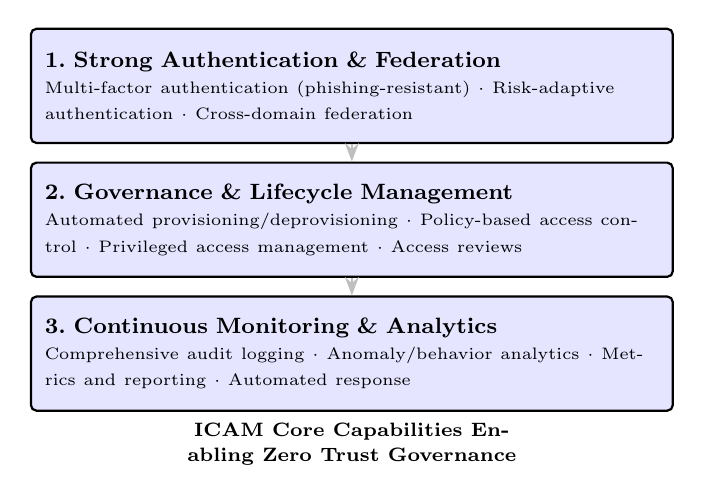
\begin{tikzpicture}[
  font=\footnotesize,
  >=Stealth,
  cbar/.style={
    rectangle, rounded corners=2pt, draw, thick,
    minimum width=8.0cm, minimum height=1.45cm,
    align=left, text width=7.8cm, inner sep=5pt,
    fill=blue!10
  },
  arr/.style={-{Stealth}, thick, gray!50}
]
  \node[cbar] (c1) at (0, 0.00) {
    \textbf{1.\ Strong Authentication \& Federation}\\
    \fontsize{6.5pt}{8pt}\selectfont
    Multi-factor authentication (phishing-resistant) $\cdot$
    Risk-adaptive authentication $\cdot$ Cross-domain federation
  };
  \node[cbar] (c2) at (0,-1.70) {
    \textbf{2.\ Governance \& Lifecycle Management}\\
    \fontsize{6.5pt}{8pt}\selectfont
    Automated provisioning/deprovisioning $\cdot$ Policy-based access control $\cdot$
    Privileged access management $\cdot$ Access reviews
  };
  \node[cbar] (c3) at (0,-3.40) {
    \textbf{3.\ Continuous Monitoring \& Analytics}\\
    \fontsize{6.5pt}{8pt}\selectfont
    Comprehensive audit logging $\cdot$ Anomaly/behavior analytics $\cdot$
    Metrics and reporting $\cdot$ Automated response
  };
  \draw[arr] (c1.south)--(c2.north);
  \draw[arr] (c2.south)--(c3.north);
  \node[font=\fontsize{7pt}{9pt}\selectfont\bfseries, text width=8.0cm, align=center]
    at (0,-4.55) {ICAM Core Capabilities Enabling Zero Trust Governance};
\end{tikzpicture}
\caption{Three core ICAM capability areas supporting Zero Trust Architecture governance.
  Each layer provides essential functions enabling continuous verification, least privilege
  enforcement, and risk-based access control.}
\label{fig:icam_capabilities}
\end{figure}

\section{Centralized vs.\ Federated Identity Structures}

\subsection{Centralized Identity Architecture}

Centralized architecture establishes a single authoritative identity provider serving as
source of truth for all users. Advantages: strong governance control; simplified
administration; enhanced monitoring visibility; reduced attack surface; and easier
compliance demonstration. Disadvantages: single point of failure requiring high
availability; scalability constraints; limited flexibility for diverse business units;
integration challenges with legacy systems; and insider threat concentration among
administrators.

\subsection{Federated Identity Architecture}

Federated architecture establishes trust relationships among multiple identity providers.
Advantages: organizational autonomy; distributed authentication load enabling scalability;
operational flexibility across diverse requirements; reduced credential proliferation; and
distributed risk. Disadvantages: governance complexity across distributed policy
enforcement; trust dependencies on partner IdP security standards; attribute exchange
privacy challenges; incident response complexity spanning organizations; and
interoperability maintenance requirements.

\subsection{Hybrid Approaches}

Many organizations implement hybrids: centralized internal identity with external
federation for cloud services and partners; hierarchical federation among autonomous
divisions with corporate minimum security standards; or progressive migration from
fragmented systems toward centralized architecture.

\subsection{Decision Framework}

%%
%% FIGURE 4 — Centralized vs Federated Identity Decision Framework (REDESIGNED)
%%
%% ORIGINAL PROBLEM:
%%   • 5 factor nodes in a single row using right= chaining → width ≈ 18 cm
%%   • Two 7.5 cm outcome boxes: cent anchored to d1 (x≈0), fed anchored to d4 (x≈12.6)
%%     → fed right edge ≈ 16+ cm, total figure ≈ 18+ cm (overflows column)
%%   • d5 (Resource Capacity, x≈16.8) wired to cent (x≈0): arrow crossed entire figure
%%
%% FIX: Two-column layout — factors split by their favoured outcome.
%%   Left col  (→ Centralized): Org Structure, Regulatory, Resource Capacity
%%   Right col (→ Federated):   Trust Model, Technical Maturity
%%   Chain arrows flow vertically within each column → outcome box.
%%   No crossing arrows. Total width ≈ 13.6 cm ✓ (IEEE figure* ≈ 18 cm)
%%
\begin{figure*}[!t]
\centering
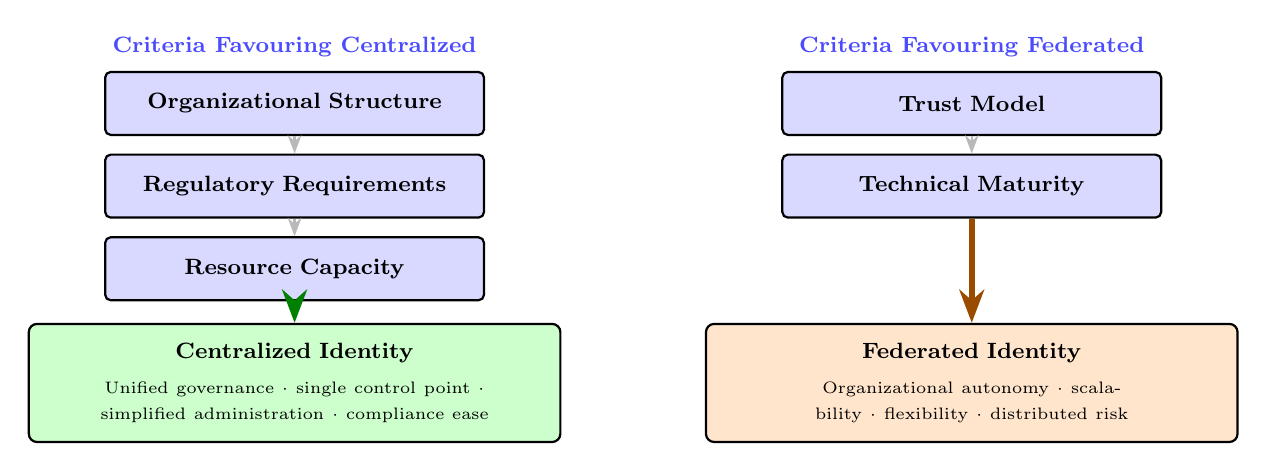
\begin{tikzpicture}[
  font=\footnotesize,
  >=Stealth,
  fbox/.style={
    rectangle, rounded corners=2pt, draw, thick,
    minimum width=4.8cm, minimum height=0.80cm,
    text centered, text width=4.6cm, inner sep=3pt,
    fill=blue!15
  },
  obox/.style={
    rectangle, rounded corners=3pt, draw, thick,
    minimum width=6.6cm, minimum height=1.5cm,
    text centered, text width=6.4cm, inner sep=5pt
  },
  arr/.style={-{Stealth}, thick, gray!55},
  harr/.style={-{Stealth}, line width=2pt}
]

  %% Column centres (gap between right edge of cent and left edge of fed ≈ 1.0cm)
  \def\xl{-4.3}   %% Left  col, centre x
  \def\xr{ 4.3}   %% Right col, centre x

  %% ── Column header labels ─────────────────────────────────────────────────
  \node[font=\footnotesize\bfseries, text=blue!70] at (\xl, 0.72)
    {Criteria Favouring Centralized};
  \node[font=\footnotesize\bfseries, text=blue!70] at (\xr, 0.72)
    {Criteria Favouring Federated};

  %% ── Left column (three factors) ──────────────────────────────────────────
  \node[fbox] (f1) at (\xl,  0.00) {\textbf{Organizational Structure}};
  \node[fbox] (f2) at (\xl, -1.05) {\textbf{Regulatory Requirements}};
  \node[fbox] (f5) at (\xl, -2.10) {\textbf{Resource Capacity}};
  \draw[arr] (f1.south)--(f2.north);
  \draw[arr] (f2.south)--(f5.north);

  %% ── Right column (two factors) ───────────────────────────────────────────
  \node[fbox] (f3) at (\xr,  0.00) {\textbf{Trust Model}};
  \node[fbox] (f4) at (\xr, -1.05) {\textbf{Technical Maturity}};
  \draw[arr] (f3.south)--(f4.north);

  %% ── Outcome boxes ─────────────────────────────────────────────────────────
  \node[obox, fill=green!20] (cent) at (\xl,-3.55) {
    \textbf{Centralized Identity}\\[3pt]
    \fontsize{6.5pt}{8pt}\selectfont
    Unified governance $\cdot$ single control point $\cdot$
    simplified administration $\cdot$ compliance ease
  };
  \node[obox, fill=orange!20] (fed) at (\xr,-3.55) {
    \textbf{Federated Identity}\\[3pt]
    \fontsize{6.5pt}{8pt}\selectfont
    Organizational autonomy $\cdot$ scalability $\cdot$
    flexibility $\cdot$ distributed risk
  };

  %% ── Terminal arrows: bottom factor → outcome ──────────────────────────────
  \draw[harr, color=green!50!black]  (f5.south) -- (cent.north);
  \draw[harr, color=orange!60!black] (f4.south) -- (fed.north);

\end{tikzpicture}
\caption{Decision framework for selecting centralized versus federated identity
  architecture. Organizational structure, regulatory requirements, and resource capacity
  favour centralized identity; trust model complexity and technical maturity favour
  federated identity. Organizations should evaluate all factors and consider hybrid
  approaches when requirements span both columns.}
\label{fig:identity_decision}
\end{figure*}

Organizations favour \textbf{centralized} architecture when: a unified organizational
structure and strong central governance exist; stringent regulations require demonstrable
policy consistency (HIPAA, PCI-DSS); all users are employees or directly managed
contractors; and adequate resources exist to implement high-availability infrastructure.
Organizations favour \textbf{federated} architecture when: autonomous business units or
extensive partner ecosystems exist; cross-organizational data sharing restrictions apply;
multiple independent organizations require collaboration; and the environment is
cloud-native with advanced identity expertise. NASA's Zero Trust implementation
exemplifies appropriate federated use: diverse centers, extensive contractor
relationships, and international partnerships requiring flexible
collaboration~\cite{pingidentity2024}.

\section{Zero Trust Adoption for Small and Medium Enterprises}

\subsection{SME-Specific Challenges}

Chang et al.~\cite{chang2025mind} identify leadership awareness as the most significant
barrier in SMEs. Misperceptions include viewing Zero Trust as applicable only to large
enterprises, incomplete understanding of business impact from cyber incidents, and a
technology-centric view neglecting policy and cultural changes. Resource constraints
manifest as financial limitations, personnel capacity shortfalls, and technical expertise
gaps. Managed security service providers offer a cost-effective path to capabilities SMEs
cannot build internally.

\subsection{Graduated Implementation Strategy}

Pawar and Palivela~\cite{pawar2023importance} demonstrate substantial risk reduction from
foundational controls before advancing to sophisticated capabilities.

\textbf{Tier 1 --- Foundation (Months 1--6)}: MFA for all remote and administrative
access; cloud-based identity provider (Microsoft 365, Google Workspace, Okta); asset
inventory identifying crown jewels; comprehensive access review removing orphaned
accounts; and basic authentication/administrative logging. Estimated investment:
\$10,000--\$30,000.

\textbf{Tier 2 --- Enhancement (Months 7--12)}: Conditional access policies enforcing
device compliance and location-based risk; just-in-time privileged access; EDR deployment;
network micro-segmentation; and security awareness training with phishing simulation.
Additional investment: \$20,000--\$50,000.

\textbf{Tier 3 --- Maturity (Year 2+)}: Data loss prevention; advanced threat protection;
Zero Trust Network Access replacing VPN; 24/7 managed detection and response; and supply
chain security extending Zero Trust to vendors. Additional investment:
\$30,000--\$70,000/year.

\subsection{Cost-Benefit Justification}

For an SME with \$10M revenue and 50 employees: 30\% annual incident probability at
\$250,000 estimated cost produces \$75,000 expected annual loss. Tier 1 investment of
\$25,000 (first year) with 60--70\% risk reduction (per FAIR Institute data) reduces
expected loss to \$26,250, yielding net first-year benefit of approximately
\$48,750~\cite{fairinstitute2025,campos2025safeguarding}.

\section{Implementation Considerations}

Critical success factors include: executive sponsorship ensuring resource allocation and
cross-functional commitment; clear policy frameworks governing access control principles
and authentication requirements; user experience balance through risk-adaptive controls
rather than blanket restrictions; incremental implementation demonstrating early wins;
and metrics enabling continuous improvement (MFA adoption, policy violations, access
review completion, mean time to detect).

Common pitfalls to avoid: technology-first purchasing without architectural principles;
attempting comprehensive simultaneous deployment; neglecting legacy system integration;
insufficient change management leading to user workarounds; and treating initial
implementation as complete rather than as the start of continuous improvement.

\section{Future Research Directions}

Priority areas include: quantitative effectiveness studies measuring Zero Trust's impact
on incident frequency and severity; SME-specific frameworks with simplified assessment
tools; AI/ML integration for risk-adaptive authentication and automated policy
generation; Zero Trust application to operational technology and IoT with
resource-constrained devices; post-quantum cryptography migration strategies for
existing deployments; and human factors research on cognitive burden and optimal
authentication friction.

\section{Conclusion}

This paper has presented a comprehensive framework for implementing ICAM-enabled Zero
Trust Architecture. Key contributions include a risk-based scope definition methodology
beginning with crown jewel identification; analysis of ICAM capabilities enabling Zero
Trust governance through authentication, lifecycle management, and continuous monitoring;
comparative evaluation of centralized versus federated identity structures with explicit
decision criteria; and graduated SME implementation strategies demonstrating positive ROI
at manageable cost.

The evidence base supports four core conclusions. First, phased, risk-based
implementation outperforms comprehensive simultaneous deployment---achieving meaningful
risk reduction while building expertise and demonstrating business value. Second, ICAM is
not merely supportive of Zero Trust but its operational foundation; without robust
identity governance, ``never trust, always verify'' remains aspirational. Third,
centralized and federated identity architectures are not universally superior; the
optimal choice depends on organizational structure, regulatory requirements, trust model,
and resource capacity, with hybrid approaches often optimal. Fourth, Zero Trust adoption
requires executive sponsorship, clear policy, and cultural change---technology alone
proves insufficient.

In a perimeter-less world where identity is the new perimeter, trust must be continuously
earned rather than implicitly granted. The framework presented here provides actionable
guidance for organizations across the maturity spectrum to progress toward that goal
incrementally, measurably, and in alignment with business objectives.

\bibliographystyle{IEEEtran}
\begin{thebibliography}{20}

\bibitem{rose2020zero}
S.~Rose, O.~Borchert, S.~Mitchell, and S.~Connelly, ``Zero Trust Architecture,''
NIST SP~800-207, Aug.~2020. \url{https://doi.org/10.6028/NIST.SP.800-207}

\bibitem{pingidentity2024}
Ping Identity, ``Zero Trust Architecture Starts with Modern ICAM,'' White Paper, 2024.
\url{https://hub.pingidentity.com/white-papers/3557-zero-trust-architecture-modern-icam}

\bibitem{shimizu2025vulnerability}
K.~Shimizu and Y.~Hashimoto, ``Vulnerability Management Chaining,'' \textit{Comput.\
Secur.}, vol.~146, p.~103188, 2025.

\bibitem{fairinstitute2025}
FAIR Institute, ``2025 State of Cyber Risk Management Report,'' June 2025.

\bibitem{chang2025mind}
Y.~Chang et al., ``Mind the Gap: Revealing Security Barriers Through Situational
Awareness of SME Key Decision-Makers,'' \textit{Comput.\ Secur.}, vol.~143, p.~103154,
2025.

\bibitem{campos2025safeguarding}
J.~Campos, F.~Oliveira, and L.~Pereira, ``Safeguarding the Future: Forecasting
Cybersecurity and Technology Adoption for SMEs,'' \textit{Procedia Comput.\ Sci.}, 2025.

\bibitem{pawar2023importance}
S.~A.~Pawar and H.~Palivela, ``Importance of Least Cybersecurity Controls for SMEs,''
in \textit{Smart Analytics, Artificial Intelligence and Sustainable Performance
Management}, vol.~110B. Emerald, 2023, pp.~21--53.

\bibitem{kindervag2010}
J.~Kindervag, ``Build Security Into Your Network's DNA: The Zero Trust Network
Architecture,'' Forrester Research, Nov.~2010.

\bibitem{ficam2021}
Federal CIO Council, ``Federal ICAM Architecture,'' v3.0, Sept.~2021.
\url{https://www.idmanagement.gov/}

\bibitem{cisa2024mfa}
CISA, ``Implementing Phishing-Resistant MFA,'' Fact Sheet, 2024.
\url{https://www.cisa.gov/sites/default/files/publications/fact-sheet-implementing-phishing-resistant-mfa-508c.pdf}

\bibitem{eo14028}
Executive Office of the President, ``Executive Order 14028: Improving the Nation's
Cybersecurity,'' \textit{Federal Register}, vol.~86, no.~93, May~2021.

\bibitem{omb2022}
Office of Management and Budget, ``Moving the U.S.\ Government Toward Zero Trust
Cybersecurity Principles,'' Memorandum M-22-09, Jan.~2022.

\bibitem{nist800207}
NIST, ``Zero Trust Architecture,'' SP~800-207, Aug.~2020.

\bibitem{buck2021never}
C.~Buck et al., ``Never Trust, Always Verify: A Multivocal Literature Review on Current
Knowledge and Research Gaps of Zero-Trust,'' \textit{Comput.\ Secur.}, vol.~110,
p.~102436, 2021.

\bibitem{gilman2017zero}
E.~Gilman and D.~Barth, \textit{Zero Trust Networks}. O'Reilly Media, 2017.

\bibitem{hardt2012oauth}
D.~Hardt, ``The OAuth 2.0 Authorization Framework,'' RFC~6749, IETF, Oct.~2012.

\bibitem{fido2019}
FIDO Alliance, ``FIDO2: Web Authentication (WebAuthn),'' W3C Recommendation, Mar.~2019.

\bibitem{saml2005}
S.~Cantor et al., ``Assertions and Protocols for OASIS SAML V2.0,'' OASIS Standard,
Mar.~2005.

\end{thebibliography}

\vspace{12pt}

\end{document}
